\cotefile{43}
\scanpage{1}
% printed form
\textsf{IMAG}

\textsf{INSTITUT MONTPELLIERAIN}

\textsf{ALEXANDER GROTHENDIECK}

\figure{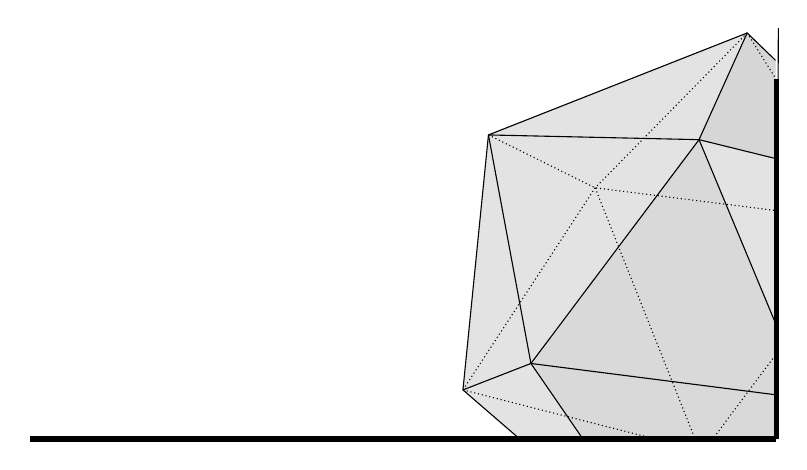
\begin{tikzpicture}[x=0.012cm,y=-0.012cm,line join=round]
\fill[gray!22] (497,139)--(771,31)--(801,60)--(801,460)--(529,460)--(470,409)--cycle;
\fill[gray!32] (771,31)--(720,144)--(801,164)--(801,60)--cycle;
\fill[gray!30] (542,381)--(720,144)--(800,336)--(800,460)--(595,458)--cycle;
\draw (497,139)--(771,31)--(801,60);
\draw (497,139)--(720,144)--(801,164);
\draw (771,31)--(720,144)--(800,336);
\draw (497,139)--(470,409)--(542,381)--(720,144);
\draw (497,139)--(542,381)--(595,458);
\draw (542,381)--(800,414);
\draw (470,409)--(529,460);
\draw[densely dotted] (497,139)--(610,195)--(801,219);
\draw[densely dotted] (771,31)--(610,195)--(470,409);
\draw[densely dotted] (610,195)--(715,459);
\draw[densely dotted] (470,409)--(662,458);
\draw[densely dotted] (736,459)--(801,372);
\draw[densely dotted] (771,31)--(801,79);
\draw (804,26)--(802,461);
\draw[line width=2pt] (802,80)--(802,461);
\draw[line width=2pt] (12,461)--(802,461);
\end{tikzpicture}}
